\documentclass{amsart}
\usepackage[margin=3cm]{geometry}                % See geometry.pdf to learn the layout options. There are lots.
\geometry{letterpaper}                   % ... or a4paper or a5paper or ...
%\geometry{landscape}                % Activate for for rotated page geometry
\usepackage[parfill]{parskip}    % Activate to begin paragraphs with an empty line rather than an indent
\usepackage{float}
\usepackage{graphicx}
\usepackage{amssymb}
\usepackage{epstopdf}
\usepackage{siunitx}
\usepackage{subcaption}
\usepackage{units}
\usepackage{setspace}

\DeclareGraphicsRule{.tif}{png}{.png}{`convert #1 `dirname #1`/`basename #1 .tif`.png}
\graphicspath{{./img/}}

\title{Electron Spin Resonance}
\author{Caspar \textsc{Lant}} % Author name

\date{\today} % Date for the report

\begin{document}

\bigskip

\maketitle % Insert the title, author and date
\begin{center}

Intermediate Experimental Physics II\\
\vspace{1.5cm}

\begin{tabular}{l r}

Section: & 001\\
\\
Date Performed: & March $e^{i\phi}$, 2016 \\ % Date the experiment was performed
Date Due: & March $ \frac{d}{dx}\delta(x)$ , 2016\\
\\
Partner: & Neil Saddler\\ % Partner names
Professor: & Prof. Andrew Kent\\
Instructor: & David Mykytyn % Instructor/supervisor
\end{tabular}
\vfill
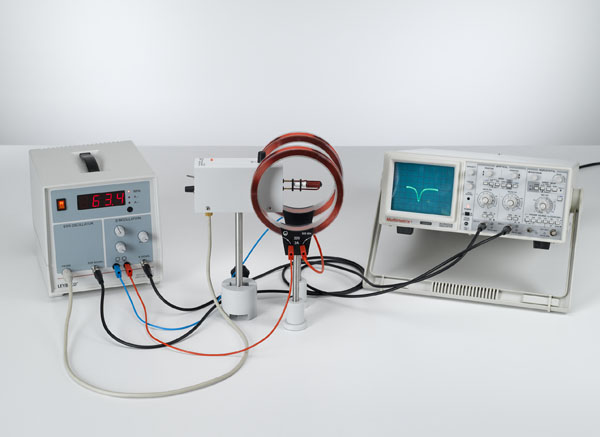
\includegraphics[width=.7\textwidth]{diagram.jpg}
\end{center}
\vfill
\pagebreak
\setstretch{1.5}
\paragraph{\textbf{The Objective} }

\section{Theoretical Background/ Abstract}
Electron Spin Resonance is a effect that occurs when materials containing unpaired electrons find themselves in the presence of an external magnetic field. Electron spin resonance is similar to the nuclear spin resonance (the subject of another experiment in this course), but instead of relating to the excited spins of atomic nuclei, this type of resonance describes the spin states of excited electrons. Depending on who you ask (and specifically their political allegiances), electron spin resonance was discovered by either a Soviet physicist by the name of Yevgeny Zavoisky, or by the Allied physicist Brebis Bleaney.\\
Electrons are partially defined by their magnetic moment and spin number, both of which are quantized. The spin number of all electrons, and fermions in general is 1/2. The magnetic moment of an electron is defined by the following:
\begin{equation}
    {\bf \mu}_S = \dfrac{g_S \mu_B S}{\hbar}
\end{equation}
Where $S$ is the electron's spin (1/2) and $g_s$ is its g-factor, which is a quantity we hope to arrive at later in this lab (but for now we'll set it equal to 2) $\mu_s$ is the Bohr magneton, equal to approximately $9 \times 10^{24}$ Joules per Tesla.
% As you can see, the magnetic moment of an electron points in the same ``direction" as its spin.
The energy of an electron in the presence of and external magnetic field $B_0$ depends on the alignment of its spin magnetic moment relative to the direction of $B_0$. Uncoupled electrons in a material such as DPPH (2,2-diphenyl-1-picrylhydrazyl, shown in figure \ref{fig:DPPH}) have little trouble setting their magnetic moments either parallel or antiparallel to the magnetic field. The energy of such an electron is given by equation \ref{eq:energy}.
\begin{equation}
    E = m_sg\mu_BB_0
    \label{eq:energy}
\end{equation}
$m_s$ differs by a sign depending on it's alignment relative to $B_0$, making the difference in energy between the parallel and the antiparallel state:
\begin{equation}
    \Delta E = h\nu = g\mu_B B_0
    \label{eq:energy_diff}
\end{equation}
Where $\nu$ is the minimum frequency required to induce a state transition. This quantity, $\Delta E$ is referred to as the ``line width", and is related to factors such as the dipole-dipole interactions between uncoupled electrons' magnetic moments, as well as the interactions between a single electron and the internal magnetic fields intrinsic to the material.
\begin{equation}
    V_s = \dfrac{h}{\rm e} \nu - \dfrac{\phi}{\rm e}
\end{equation}
In DPPH it is electron exchange which is important. The full width at half height of the resonance in terms of the magnetic field will be called $\delta B$ and will be measured.
\begin{equation}
    \vec \mu \times \vec B = \omega_L \times \vec L
\end{equation}

\begin{equation}
    \dfrac{\mu_0 N}{2R}\left(\dfrac{4}{5}\right)^{\frac{3}{2}}(2I_0) = 2.115(2I_0)mT
\end{equation}

\section{Experimental Procedure}
\begin{enumerate}
    \item Plug everything in in the manner depicted in the illustration on the cover page and ensure that all measurement devices are powered off.
    \item Carefully plug the largest RF coil into the RF unit.
    \item space the solenoids by a distance of 6.8cm.
    \item Place the sample into the coil and place it in the center of the volume formed by each solenoid.
    \item Make sure that $U_0$ is set to zero, and $U_{\rm mod}$ is set to the second scale marking.
    \item Turn on all devices. The oscilloscope should be set for two channel operation with channel one triggering.
    \item Set the frequency adjuster on the RF unit to 15 MHz. The Amplitude should be at its maximum.
    \item Now, increase the DC coil voltage $U_0$ until resonances are seen on the oscilloscope's phosphor screen. This will take the form of a nice, symmetric ``v"-curve, similar to the Gaussian function $-e^{-x^2/a}$
    \item Note the current
\end{enumerate}

\section{Graphs and Tables}

\begin{table}[H]
    \centering
    \caption{Voltage vs. Deflection}
    \bigskip \bigskip
    \label{table:deflection}
    \begin{tabular}{c|c|c|c}
        $f$ (MHz)&$I_0$ (A) &$2I_0$ (A) &$B$(mT) \\
        30.7     & 0.644    & 1.288     & 2.724  \\
        35.0     & 0.731    & 1.462     & 3.092  \\
        40.0     & 0.880    & 1.760     & 3.722  \\
        45.0     & 0.993    & 1.986     & 4.200  \\
        50.0     & 1.112    & 2.224     & 4.704  \\
        55.0     & 1.205    & 2.410     & 5.097  \\
        60.0     & 1.317    & 2.634     & 5.571  \\
        65.0     & 1.442    & 2.884     & 6.100  \\
        70.0     & 1.534    & 3.068     & 6.489  \\
        75.0     & 1.595    & 3.190     & 6.747  \\
        80.0     & 1.692    & 3.384     & 7.157  \\
        85.0     & 1.765    & 3.530     & 7.466  \\
        90.0     & 1.917    & 3.834     & 8.109  \\
        95.0     & 2.035    & 4.070     & 8.608  \\
        100.0    & 2.067    & 4.134     & 8.743  \\
        105.0    & 2.221    & 4.442     & 9.395  \\
        110.0    & 2.293    & 4.586     & 9.699  \\
        100.0    & 2.412    & 4.824     & 10.203
    \end{tabular}
\end{table}
%
% \begin{minipage}{.5\textwidth}
%     \centering
%     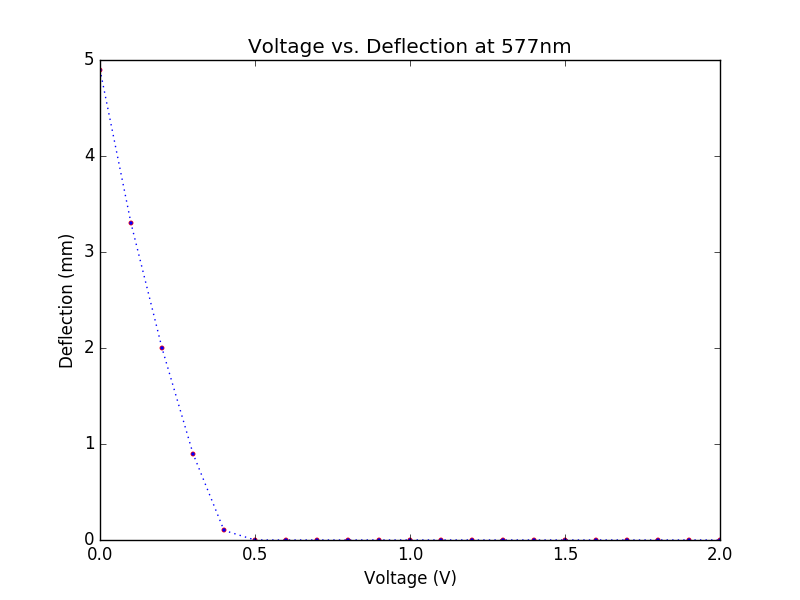
\includegraphics[height=.23\textheight]{577.png}\\
%     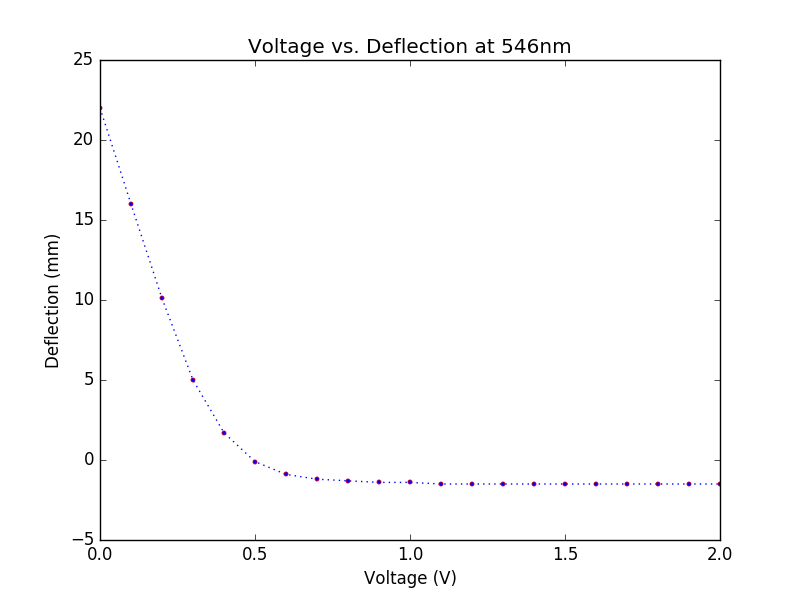
\includegraphics[height=.23\textheight]{546.png}\\
%     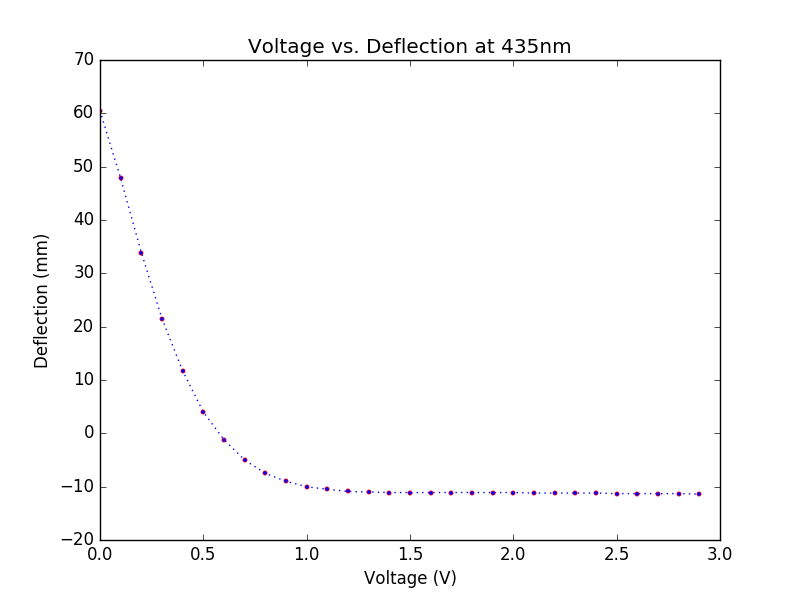
\includegraphics[height=.23\textheight]{435.png}
% \end{minipage}
% \end{table}

\begin{figure}
    \centering
    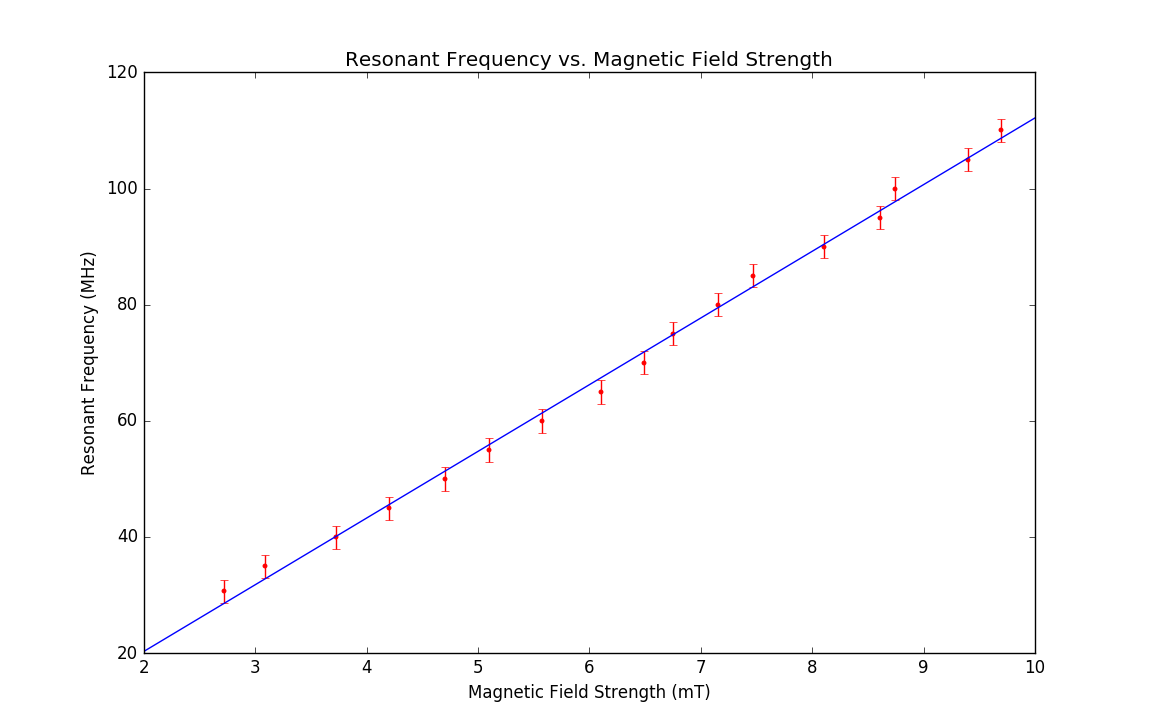
\includegraphics[width=\textwidth]{fitted.png}
    \caption{Finding $g_s$}
\end{figure}

\begin{figure}
    \centering
    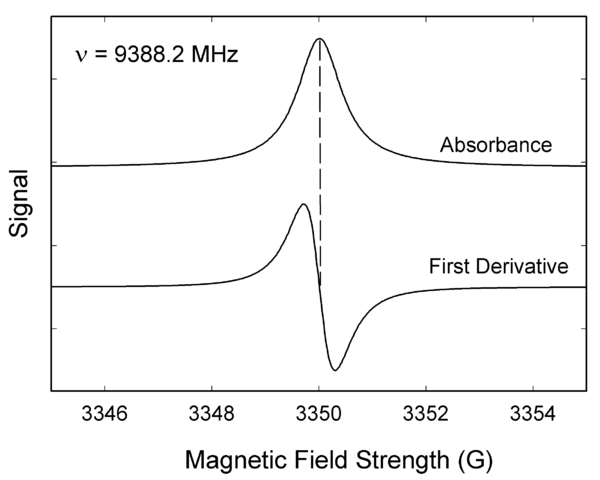
\includegraphics[width=0.8\textwidth]{lines.png}
    \caption{Schematic Diagram of the Experimental Setup}
\end{figure}


\begin{figure}
    \begin{minipage}{.45\textwidth}
        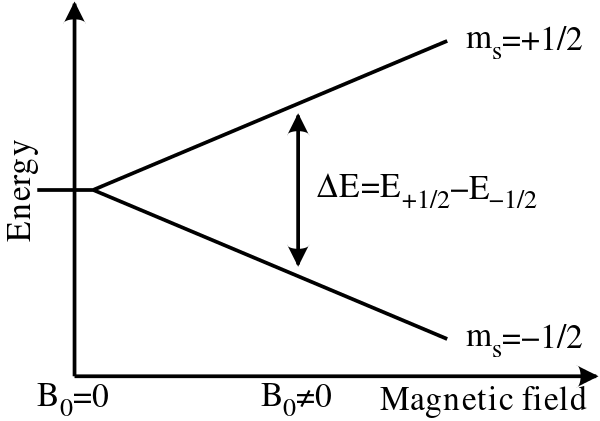
\includegraphics[width=\textwidth]{splitting.png}
    \end{minipage}
    %
    \begin{minipage}{.45\textwidth}

    \end{minipage}
\end{figure}

The topmost plot corresponds to a filter of slit width 577 nm, the middle plot 546 nm, and the last plot a wavelength of 435 nm.
\section{Questions}

\begin{enumerate}
    \item {\textit{The manufacturer designed this experiment with the coils connected in parallel. A series connection would be better. Why?}
    \begin{quote}

    \end{quote}}
    \item {\textit{The p-p modulation current $\delta(2I_0)$ for the half-width $\delta$B is obtained from  Where does the divisor 10 come from?}
    \begin{quote}

    \end{quote}}
    \item {\textit{In the method given for measuring $\delta$B, the scope controls are not used in a calibrated mode. Why is this OK?}
    \begin{quote}

    \end{quote}}
    \item {\textit{Why is the multimeter set for DC amperes for measuring g and for AC amperes for measuring the line width?}
    \begin{quote}
        The line width is given by $I_{\rm rms}$, which
    \end{quote}}
    \item {\textit{Is there an RF electric field associated with the RF coil? If so, make a sketch of what the fields look like.}
    \begin{quote}
        There is no electric field associated with the RF coil, assuming it's been aligned properly.
    \end{quote}}



\end{enumerate}

\section{Error Analysis}


slope = 11.4794866225

\end{document}
